\documentclass[a4paper, 11pt]{article}
\usepackage[utf8]{inputenc}
\usepackage[scaled]{helvet}
\renewcommand\familydefault{\sfdefault}
\usepackage[T1]{fontenc}
\usepackage[francais]{babel}
\usepackage[left=2.2cm,top=2.2cm,right=2.2cm,bottom=2.2cm]{geometry}
\usepackage{graphicx}
\usepackage{authblk}
\usepackage{enumitem}
\usepackage{listings} 
\usepackage{minted}
\usepackage{hyperref} 
\hypersetup{
	colorlinks,
	citecolor=black,
	filecolor=black,
	linkcolor=black,
	urlcolor=blue
}

\begin{document}

\title{La boule qui tombe... qui tombe...} 
\author{Raed Abdennadher} 
\affil{\small Développement mobile android - Prof Stephane Malandain} 
\affil{\small Hepia ITI 3\up{ème} année} 
\maketitle

\section{Introduction}
Le but de ce tp est de réaliser un jeu android :
\begin{itemize}
	\item L'objectif du jeu est de gagner le plus de points possible.
	\item Une boule apparaît en haut de l’écran et commence à tomber sous l'éffet de la gravité tant qu'il n'y a pas
	de plateformes horizontaux qui s'opposent à son mouvement vertical (du haut vers le bas). A noter que la masse
	de la boule est variable selon le mode du jeu. Par exemple, dans le mode facile, la boule est relativement
	légère, et donc sa vitesse de chute est relativement moins rapide que celle dans le mode difficile.
	\item Dans les plateformes il y a des trous à travers desquels la boule peut tomber.
	\item En commençant une partie, un timer se lance. Il faut que la boule arrive en bas de l'écran avant que
	le temps échu.
	\item Sur l'espace du jeu, il y a des bonus et des malus (selon la difficulté du jeu) : un bonus (en verts)
	ajoute 5 secondes au timer, alos qu'un malus (en rouge) enlève 5 secondes du timer. Quand l'utilisateur choisit
	le mode facile, il y aura que des bonus dans le jeu. Pour le mode intermédière il y a des bonus et des malus.
	Dans le mode difficile, il y a que des malus.
	\item En bas de l'écran, il y a des cases. Chaque case contient un nombre de points différent et aléatoire.
\end{itemize}

\section{Architecture du projet}
\subsection{Architecture générale}
Pour notre site web, nous avons choisi une architecture 3 tiers qui comporte 3 couches : 
\begin{itemize}
	\item Couche "Présentation" : c'est l'interface graphique à traver de laquelle l'utilisateur va pouvoir intéragir avec le site web.
	\item Couche "Métier" : c'est la partie responsable de tous les calculs et les traitements de données qui se passent en arrière plan.
	\item Couche "Base de données" : ici on a les scripts postgreSQL qui permettent l'interrogation avec la base de données.
\end{itemize}
La figure \ref{fig:architecture} représente l'architecture du projet.

\begin{figure}[!ht]
	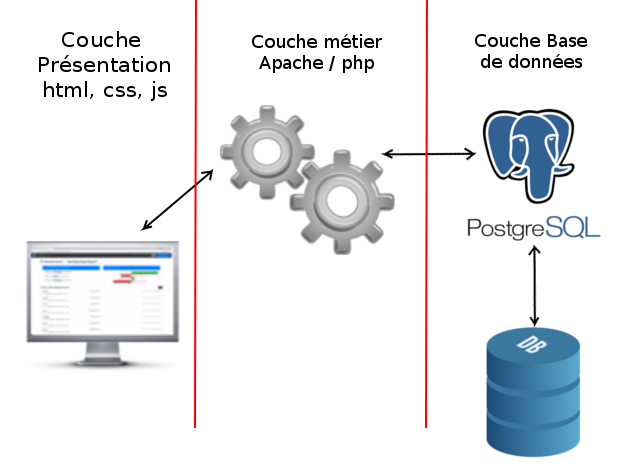
\includegraphics[scale=.9]{images/architecture.png}
	\caption{Modèle relationnel de la base de données}
	\label{fig:architecture}
\end{figure}

\subsection{Base de données}
La figure \ref{fig:model_db} représente le modèle relationnel de la base de données de notre site web.
\begin{figure}[!ht]
	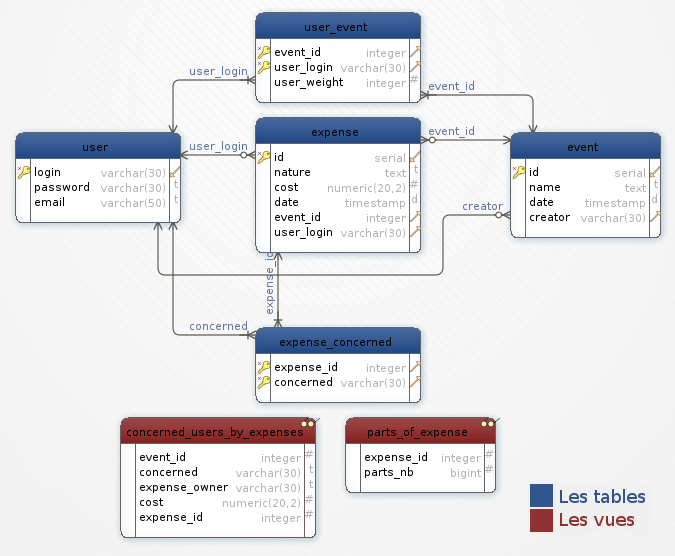
\includegraphics[scale=.8]{images/db.png}
	\caption{Modèle relationnel de la base de données}
	\label{fig:model_db}
\end{figure}

\section{Technologies et outils}

\subsection{Technologies utilisées}
Nous avons utilisé les technologies suivantes :
\begin{itemize}
	\item HTML5, CSS3, \href{http://getbootstrap.com/}{Bootstrap V4}, \href{https://jquery.org/}{jQuery 3.2}, 
	\href{https://jqueryui.com/}{jQuery UI 1.12}, \href{http://akquinet.github.io/jquery-toastmessage-plugin/}{jquery-toastmessage-plugin} pour la couche présentation et construction de l'interface graphique de notre site web.
	\item php7.0 et JavaScript(ES6) pour la couche métier de notre site web (les connexions à la base de données, les
	calculs, affichage dynamique en fonction des données...)
	\item \href{https://www.postgresql.org/}{PostgreSQL 9.6.4} pour la couche base de données
\end{itemize}

\subsection{Explication des choix}
Dans cette section, nous allons expliquer pourquoi nous avons choisi PostgreSQL pour la base de données et Bootstrap pour le design du site.
\paragraph{} Pendant la phase de conception de notre site web, nous avons remarqué que nous aurons besoin d'utiliser les triggers pour la cause suivante : au moment de l'insertion d'une nouvelle dépense, il faut vérifier si les utilisateurs concernés appartiennent bien au groupe de l'évènement. Et vu que nous avons déjà eu un cours de base de données en PostgreSQL l'année dernière, nous voulions utiliser cette technologie pour appliquer ce qu'on avait appris.
\paragraph{} En ce qui concerne Bootstrap, nous trouvons que c'est un très bon outil qui permet de faciliter la création du design du site. Il offre des mises en forme responsive en ajoutant simplement une classe css à une balise html par exemple.

\section{Structure du projet}
Nous avons organisé notre projet de la façon suivante :
\begin{itemize} 
	\item Le script de la création de la base de donées se trouve sous le dossier $psql$. Une documentation pour la base de données est aussi disponible (sous forme html) sous le même dossier.
	\item Les fichiers CSS se trouvent sous de dossier $css$
	\item Les fichiers JavaScript se trouvent sous de dossier $js$
	\item Les icons se trouvent sous de dossier $icons$
	\item Les images se trouvent sous de dossier $images$
	\item Les fichiers PHP se trouvent directement sous la racine
\end{itemize}
Dans le fichier $Session.php$ on a la gestion de session : connecter un utilisateur et ouvrir une session, fermer une session et récupérer la session en cours. Les fonctions pour la connexion à la base de données se trouvent dans le fichier $Connexion.php$ (Remarque : en lisant la documentation de php pour la fonction $pg\_connect$, on a constaté que nous avons pas besoin d'appliquer le parton de conception $singletant$ car cette fonction offre la même logique. C'est à dire, si une connexion à la même base de données est ouverte, elle va pas créer une nouvelle). Les fonction qui permettent de communiquer directement avec la base de données sont dans le fichier $Functions.php$.
\newline Au début de chaque page affichée dans le navigateur, toutes ces fonctions sont chargées via le bout de code dans le fichier $includes.php$.

\section{Procédure d'installation}
Afin de reprendre le projet, il faut :
\begin{itemize}
	\item Installer un serveur appache (version 2.4.25)
	\item Installer php (version 7)
	\item Installer PostgreSQL (version 9.6.4). Remarque : l'installation de PostgreSQL crée automatique un utilisateur unix "postgres" qui va être le super utilisateur du serveur PostgreSQL.
	\item Une fois ces outils sont installés, on doit créer un utilisateur postgres pour la connexion à la base de données. Dans la console, entrez les commandes suivantes :
	\begin{itemize}
		\item Se logger en tant que super utilisateur postgres : 
			\newline$\# $\mintinline{sh}{su - postgres}
		\item Se connecter su serveur PostgreSQL : 
			\newline$\$ $\mintinline{sh}{psql template1}
		\item Ajouter un utilisateur ayant le même nom que votre utilisateur unix courant (Attention, si vous saisissez un nom différent, la connexion aura pas lieu après) : 
			\newline$template1=\# $\mintinline{psql}{CREATE USER 'myUserName' WITH PASSWORD 'myPassword';}
		\item Créer une base de données nommée "trip" : 
			\newline$template1=\# $\mintinline{psql}{CREATE DATABASE trip;}
		\item Donner tout les droits à l'utilisateur qu'on vient de créer :
			\newline$template1=\# $\mintinline{psql}{GRANT ALL PRIVILEGES ON DATABASE trip to 'myUserName';}
		\item Quitter : 
			\newline$template1=\# $\mintinline{psql}{\q}
		\item Après avoir préparé l'environnement de PostgreSQL, vous devez changer les variables de connexion dans le fichier $Connexion.php$ (ligne 7 et 8) :
			\newline \mintinline{php}{define('USER', 'myUserName');}
			\newline \mintinline{php}{define('PASSWORD', 'myPassword');}
		\item Maintenant, se connecter en tant que "myUserName" à la base de données via la console :
			\newline$\$ $\mintinline{sh}{su - myUserName}
			\newline$\$ $\mintinline{sh}{psql -d trip -U myUserName}
		\item Créer un schéma sous le nom "trip" :
			\newline$myUserName=>$\mintinline{psql}{CREATE SCHEMA trip;}
		\item Finalement, excécuter le script $script\_psql.sql$ :
			\newline$myUserName=>$\mintinline{psql}{\i script_psql.sql}
	\end{itemize}
\end{itemize}

\section{Conclusion}
Grace à ce mini-projet, nous avons pu appliquer beaucoup de connaissances théorique qu'on avait vu en cours pendant l'année dernière, et nous a permet de bien métriser l'intégration des différentes technologies afin d'aboutir à un produit qui fonctionne.

\end{document}
